\chapter{Elastic Constants}
\label{section:elasticconstantsappendix}


\section{Elastic Constant Matrices}

\renewcommand{\arraystretch}{1.7}
\begin{table}[!htbp]
\begin{tabular}{ll}
Crystal: & Cubic \\
Sides: & a = b = c \\
Angles: & $\alpha = \beta = \gamma = \frac{\pi}{2} \text{radians}$ \\
Symmetry: & $\frac{\pi}{2} \text{radians}$ rotation, 3 mutually orthogonal planes of symmetry \\
No. Independent Elastic Constants: & 3  \\
Elastic Constants: & $ \begin{bmatrix} C_{11} & C_{12} & C_{12} & 0 & 0 & 0 \\ C_{12} & C_{11} & C_{12} & 0 & 0 & 0 \\ C_{12} & C_{12} & C_{11} & 0 & 0 & 0 \\ 0 & 0 & 0 & C_{44} & 0 & 0 \\ 0 & 0 & 0 & 0 & C_{44} & 0 \\ 0 & 0 & 0 & 0 & 0 & C_{44} \end{bmatrix} $ \\
\end{tabular}
\label{tab:elasticcubic}
\caption{Independent elastic constants for a cubic crystal\cite{typesofelasticstrain}}
\end{table}


\renewcommand{\arraystretch}{1.7}
\begin{table}[!htbp]
\begin{tabular}{ll}
Crystal: & Orthorhombic/Orthotropic \\
Sides: & $a \ne b \ne c$ \\
Angles: & $\alpha = \beta = \gamma = \frac{\pi}{2} \text{radians}$ \\
Symmetry: & 3 mutually orthogonal planes of symmetry \\
No. Independent Elastic Constants: & 9  \\
Elastic Constants: & $\begin{bmatrix} C_{11} & C_{12} & C_{13} & 0 & 0 & 0 \\ C_{12} & C_{22} & C_{23} & 0 & 0 & 0 \\ C_{13} & C_{23} & C_{33} & 0 & 0 & 0 \\ 0 & 0 & 0 & C_{44} & 0 & 0 \\ 0 & 0 & 0 & 0 & C_{55} & 0 \\ 0 & 0 & 0 & 0 & 0 & C_{66} \end{bmatrix} $ \\
\end{tabular}
\label{tab:elasticorthorhombic}
\caption{Independent elastic constants for an orthorhombic/orthotropic crystal\cite{typesofelasticstrain}}
\end{table}


\renewcommand{\arraystretch}{1.7}
\begin{table}[!htbp]
\begin{tabular}{ll}
Crystal: & Monoclinic \\
Sides: & $a \ne b \ne c$ \\
Angles: & $\alpha < \frac{\pi}{2} \text{radians},  \beta = \gamma = \frac{\pi}{2} \text{radians}$ \\
Symmetry: & symmetry in the xy plane \\
No. Independent Elastic Constants: & 13  \\
Elastic Constants: & $ \begin{bmatrix} C_{11} & C_{12} & C_{13} & 0 & 0 & C_{16} \\ C_{12} & C_{22} & C_{23} & 0 & 0 & C_{26} \\ C_{13} & C_{23} & C_{33} & 0 & 0 & C_{36} \\ 0 & 0 & 0 & C_{44} & C_{45} & 0 \\ 0 & 0 & 0 & C_{45} & C_{55} & 0 \\ C_{16} & C_{26} & C_{36} & 0 & 0 & C_{66} \end{bmatrix} $ \\
\end{tabular}
\label{tab:elasticmonoclinic}
\caption{Independent elastic constants for a monoclinic crystal\cite{typesofelasticstrain}}
\end{table}


\renewcommand{\arraystretch}{1.7}
\begin{table}[!htbp]
\begin{tabular}{ll}
Crystal: & Triclinic \\
Sides: & $a \ne b \ne c$ \\
Angles: & $ \alpha < \frac{\pi}{2} \text{radians}, \beta < \frac{\pi}{2} \text{radians}, \gamma < \frac{\pi}{2} \text{radians} $ \\
Symmetry: & no symmetry \\
No. Independent Elastic Constants: & 21  \\
Elastic Constants: & $ \begin{bmatrix} C_{11} & C_{12} & C_{13} & 0 & 0 & C_{16} \\ C_{12} & C_{22} & C_{23} & 0 & 0 & C_{26} \\ C_{13} & C_{23} & C_{33} & 0 & 0 & C_{36} \\ 0 & 0 & 0 & C_{44} & C_{45} & 0 \\ 0 & 0 & 0 & C_{45} & C_{55} & 0 \\ C_{16} & C_{26} & C_{36} & 0 & 0 & C_{66} \end{bmatrix} $ \\
\end{tabular}
\label{tab:elastictriclinic}
\caption{Independent elastic constants for a triclinic crystal\cite{typesofelasticstrain}}
\end{table}


\FloatBarrier
\section{Sets of Strains Applied to Calculate Elastic Constants}

Strains are applied to a relaxed cell to determine the elastic constants.  Various methods have been used, and these differ from paper to paper based on the crystal structure and the author.  Several of these strains have been used throughout this work in various computer codes, including the QE\_EOS and EAMPA codes.

\subsection{Cubic Crystals - Mehl, Singh, Klein and Papaconstantopoulos 1993}

\renewcommand{\arraystretch}{1.7}
\begin{table}[!htbp]
\centering
%\begin{adjustbox}{width=1\textwidth}
\begin{tabular}{c c c c c c c}
\hline\hline
$e_1$ & $e_2$ & $e_3$ & $e_4$ & $e_5$ & $e_6$ & $E(\sigma)$ \\
\hline\hline
$\sigma$ & $\sigma$ & $\sigma$ & 0 & 0 & 0 & BM EoS Fit $B_0$\\
$\sigma$ & $-\sigma$ & $\frac{\sigma^2}{1 - \sigma^2}$ & 0 & 0 & 0 & $\Delta E(\sigma) = \Delta E(-\sigma) = V_{0} ((C_{11} - C_{12}) \frac{\sigma}{2} + O[\sigma^4]$ \\
0 & 0 & $\frac{\sigma^2}{4 - \sigma^2}$ & 0 & 0 & $\sigma$ & $\Delta E(\sigma) = \Delta E(-\sigma) = V_{0} C_{44} \frac{\sigma}{2} + O[\sigma^4]$ \\
\end{tabular}
%\end{adjustbox}
\label{tab:mskp1993}
\caption{Calculation of elastic constants using the equation of state, a volume conserving orthorhombic strain and volume conserving monoclinic strain.\cite{elasticpropertiesmehl}\cite{mehlsp}}
\end{table}

These values are inserted into the strain matrix in eq. \ref{eq:eqStrainMatrixMSKP}.

\begin{equation}
\begin{split}
\vec{\epsilon} = \begin{bmatrix} e_1 & \frac{e_6}{2} & \frac{e_5}{2} \\ \frac{e_6}{2} & e_2 & \frac{e_4}{2} \\ \frac{e_5}{2} & \frac{e_4}{2} & e_3 \end{bmatrix}
\end{split}
\label{eq:eqStrainMatrixMSKP}
\end{equation}

The values for $C_{11}$ and $C_{12}$ are computed using the polynomial fit to the change in energy due to the second strain and the bulk modulus.

\begin{equation}
\begin{split}
	\begin{bmatrix} 1 & -1 \\ \frac{1}{3} & \frac{2}{3} \end{bmatrix} \begin{bmatrix} C_{11} \\ C_{12} \end{bmatrix} = \begin{bmatrix} \frac{C_{p}}{V_0} \\ B_0 \end{bmatrix}
\end{split}
\label{eq:eqC11C12elastic}
\end{equation}


\subsection{Orthorhombic Crystals - Ravindran, Fast, Korzhavyi and Johansson}

\renewcommand{\arraystretch}{1.7}
\begin{table}[!htbp]
\centering
%\begin{adjustbox}{width=1\textwidth}
\begin{tabular}{c c c c c c c}
\hline\hline
$e_1$ & $e_2$ & $e_3$ & $e_4$ & $e_5$ & $e_6$ & $E(\sigma)$ \\
\hline\hline
$\sigma$ & 0 & 0 & 0 & 0 & 0 &  $E(V,\sigma) = E(V_0, 0) + V_0 \left( \tau_1 \sigma + \frac{C_{11}}{2} \sigma^2 \right) $ \\
0 & $\sigma$ & 0 & 0 & 0 & 0 &  $E(V,\sigma) = E(V_0, 0) + V_0 \left( \tau_2 \sigma + \frac{C_{22}}{2} \sigma^2 \right) $ \\
0 & 0 & $\sigma$ & 0 & 0 & 0 &  $E(V,\sigma) = E(V_0, 0) + V_0 \left( \tau_3 \sigma + \frac{C_{33}}{2} \sigma^2 \right) $ \\
$\frac{1}{(1-\sigma^2)^{\frac{1}{3}}}$ & $\frac{1}{(1-\sigma^2)^{\frac{1}{3}}}$ & $\frac{1}{(1-\sigma^2)^{\frac{1}{3}}}$ & $\frac{1}{(1-\sigma^2)^{\frac{1}{3}}}$ & 0 & 0 &  $E(V,\sigma) = E(V_0, 0) + V_0 \left(2 \tau_4 \sigma + 2 C_{44} \sigma^2 \right) $ \\
$\frac{1}{(1-\sigma^2)^{\frac{1}{3}}}$ & $\frac{1}{(1-\sigma^2)^{\frac{1}{3}}}$ & $\frac{1}{(1-\sigma^2)^{\frac{1}{3}}}$ & 0 & $\frac{1}{(1-\sigma^2)^{\frac{1}{3}}}$ & 0 &  $E(V,\sigma) = E(V_0, 0) + V_0 \left(2 \tau_5 \sigma + 2 C_{55} \sigma^2 \right) $ \\
$\frac{1}{(1-\sigma^2)^{\frac{1}{3}}}$ & $\frac{1}{(1-\sigma^2)^{\frac{1}{3}}}$ & $\frac{1}{(1-\sigma^2)^{\frac{1}{3}}}$ & 0 & 0 & $\frac{1}{(1-\sigma^2)^{\frac{1}{3}}}$ &  $E(V,\sigma) = E(V_0, 0) + V_0 \left(2 \tau_6 \sigma + 2 C_{66} \sigma^2 \right) $ \\
$\frac{1+\sigma}{(1 - \sigma^2)^{\frac{1}{3}}}$ & $\frac{1-\sigma}{(1 - \sigma^2)^{\frac{1}{3}}}$ & $\frac{1}{(1 - \sigma^2)^{\frac{1}{3}}}$ & 0 & 0 & 0 &  $E(V,\sigma) = E(V_0, 0) + V_0 \left( (\tau_1 - \tau_2) \sigma + \frac{C_{11} + C_{22} - 2 C_{12} }{2} \sigma^2 \right) $ \\
$\frac{1+\sigma}{(1 - \sigma^2)^{\frac{1}{3}}}$ & $\frac{1}{(1 - \sigma^2)^{\frac{1}{3}}}$ & $\frac{1-\sigma}{(1 - \sigma^2)^{\frac{1}{3}}}$ & 0 & 0 & 0 &  $E(V,\sigma) = E(V_0, 0) + V_0 \left( (\tau_1 - \tau_3) \sigma + \frac{C_{11} + C_{33} - 2 C_{13} }{2} \sigma^2 \right) $ \\
$\frac{1}{(1 - \sigma^2)^{\frac{1}{3}}}$ & $\frac{1+\sigma}{(1 - \sigma^2)^{\frac{1}{3}}}$ & $\frac{1-\sigma}{(1 - \sigma^2)^{\frac{1}{3}}}$ & 0 & 0 & 0 &  $E(V,\sigma) = E(V_0, 0) + V_0 \left( (\tau_2 - \tau_3) \sigma + \frac{C_{22} + C_{33} - 2 C_{23} }{2} \sigma^2 \right) $ \\
\end{tabular}
%\end{adjustbox}
\label{tab:multicol}
\caption{Calculation of orthorhombic elastic constants by Ravindran et al.\cite{dfttisiravindran}}
\end{table}


These values are inserted into the strain matrix in eq. \ref{eq:eqStrainMatrixRFKJ}.

\begin{equation}
\begin{split}
\vec{\epsilon} = \begin{bmatrix} e_1 & e_6 & e_5 \\ e_6 & e_2 & e_4 \\ e_5 & e_4 & e_3 \end{bmatrix}
\end{split}
\label{eq:eqStrainMatrixRFKJ}
\end{equation}

The 9 elastic constants are calculated by polynomial fit to the strain-energy data.  Using the second order of each polynomial, $p_1 \text{ to } p_9$, the elastic constants are calculated by solving eq \ref{eq:eqRFKJlin}. 

\begin{equation}
\begin{split}
	\begin{bmatrix} 
   \frac{V_0}{2} & 0 & 0 & 0 & 0 & 0 & 0 & 0 & 0 \\ 
   0 & \frac{V_0}{2} & 0 & 0 & 0 & 0 & 0 & 0 & 0 \\ 
   0 & 0 & \frac{V_0}{2} & 0 & 0 & 0 & 0 & 0 & 0 \\ 
   0 & 0 & 0 & 2V_0 & 0 & 0 & 0 & 0 & 0 \\ 
   0 & 0 & 0 & 0 & 2V_0 & 0 & 0 & 0 & 0 \\ 
   0 & 0 & 0 & 0 & 0 & 2V_0 & 0 & 0 & 0 \\ 
   \frac{V_0}{2} & \frac{V_0}{2} & 0 & 0 & 0 & 0 & -V_0 & 0 & 0 \\ 
   \frac{V_0}{2} & 0 & \frac{V_0}{2} & 0 & 0 & 0 & 0 & -V_0 & 0 \\ 
   0 & \frac{V_0}{2} & \frac{V_0}{2} & 0 & 0 & 0 & 0 & 0 & -V_0 \\ 
\end{bmatrix} 
\begin{bmatrix} 
C_{11} \\ 
C_{22} \\ 
C_{33} \\ 
C_{44} \\ 
C_{55} \\ 
C_{66} \\ 
C_{12} \\ 
C_{13} \\ 
C_{23} \\  
\end{bmatrix} = 
\begin{bmatrix} 
p_{1} \\ 
p_{2} \\ 
p_{3} \\ 
p_{4} \\ 
p_{5} \\ 
p_{6} \\ 
p_{7} \\ 
p_{8} \\ 
p_{9} \\  
\end{bmatrix}
\end{split}
\label{eq:eqRFKJlin}
\end{equation}



\FloatBarrier
\subsection{Cubic Crystals - Connetable and Thomas 2009}

\renewcommand{\arraystretch}{1.7}
\begin{table}[!htbp]
\centering
%\begin{adjustbox}{width=1\textwidth}
\begin{tabular}{c c c c c c c}
\hline\hline
$e_1$ & $e_2$ & $e_3$ & $e_4$ & $e_5$ & $e_6$ & $E(\sigma)$ \\
\hline\hline
$\sigma$ & $\sigma$ & $\sigma$ & 0 & 0 & 0 & BM EoS Fit $B_0$\\

$\sigma$ & 0 & 0& 0 & 0 & 0 & $\Delta E(\sigma) = \frac{V_{0}}{2} C_{11} \sigma^2 + O[\sigma^4]$ \\

0 & 0 & 0& $2 \sigma$ & $2 \sigma$ & $2 \sigma$ & $\Delta E(\sigma) = 6 V_{0} C_{44} \sigma^2 + O[\sigma^4]$ \\
\end{tabular}
%\end{adjustbox}
\label{tab:ctcubic}
\caption{Calculation of elastic constants for a cubic crystal\cite{orthonisi}}.
\end{table}


\begin{equation}
\begin{split}
\vec{\epsilon} = \begin{bmatrix} 2 e_1 & e_6 & e_5 \\ e_6 & 2 e_2 & e_4 \\ e_5 & e_4 & 2 e_3 \end{bmatrix}
\end{split}
\label{eq:eqStrainMatrixCT}
\end{equation}









\FloatBarrier
\subsection{Orthorhombic Crystals - Connetable and Thomas 2009}

\renewcommand{\arraystretch}{1.7}
\begin{table}[!htbp]
\centering
%\begin{adjustbox}{width=1\textwidth}
\begin{tabular}{c c c c c c c}
\hline\hline
$e_1$ & $e_2$ & $e_3$ & $e_4$ & $e_5$ & $e_6$ & $E(\sigma)$ \\
\hline\hline
$\sigma$ & 0 & 0 & 0 & 0 & 0 & $\Delta E(\sigma) = \frac{V_{0}}{2} C_{11} \sigma^2$ \\
0 & $\sigma$ & 0 & 0 & 0 & 0 & $\Delta E(\sigma) = \frac{V_{0}}{2} C_{22} \sigma^2$ \\
0 & 0 & $\sigma$ & 0 & 0 & 0 & $\Delta E(\sigma) = \frac{V_{0}}{2} C_{33} \sigma^2$ \\

0 & 0 & 0 & 2 $\sigma$ & 0 & 0 & $\Delta E(\sigma) = 2 V_{0} C_{44} \sigma^2$ \\
0 & 0 & 0 & 0 & 2 $\sigma$ & 0 & $\Delta E(\sigma) = 2 V_{0} C_{55} \sigma^2$ \\
0 & 0 & 0 & 0 & 0 & 2 $\sigma$ & $\Delta E(\sigma) = 2 V_{0} C_{66} \sigma^2$ \\

$u (1+\sigma) - 1$ & $u (1-\sigma) - 1$ & $u - 1$ & 0 & 0 & 0 & $\Delta E(\sigma) = \frac{V_{0}}{2} (C_{11} + C_{22} - 2 C_{12}) \sigma^2$ \\
$u (1+\sigma) - 1$ & $u - 1$ & $u (1-\sigma) - 1$ & 0 & 0 & 0 & $\Delta E(\sigma) = \frac{V_{0}}{2} (C_{11} + C_{33} - 2 C_{13}) \sigma^2$ \\
$u - 1$ & $u (1+\sigma) - 1$ & $u (1-\sigma) - 1$ & 0 & 0 & 0 & $\Delta E(\sigma) = \frac{V_{0}}{2} (C_{22} + C_{33} - 2 C_{23}) \sigma^2$ \\

\end{tabular}
%\end{adjustbox}
\label{tab:ctcubic}
\caption{Calculation of elastic constants for a cubic crystal\cite{orthonisi}, $u = (1-\sigma^2)^{-\frac{1}{3}}$}.
\end{table}


\begin{equation}
\begin{split}
\vec{\epsilon} = \begin{bmatrix} 2 e_1 & e_6 & e_5 \\ e_6 & 2 e_2 & e_4 \\ e_5 & e_4 & 2 e_3 \end{bmatrix}
\end{split}
\label{eq:eqStrainMatrixCT}
\end{equation}


\subsection{Stability Conditions}
\label{section:stabilityconditions}

Whilst the elastic constants may be computed using first-principles calculations, there are a series of assumptions and approximations made in order to solve first-principles calculations in a reasonable amount of time.  There must be a sanity check, as it is no use to compute the elastic constants from \acrshort{dft} to find the crystals are unstable.

For a cubic crystal with three independent elastic constants and zero stress, the Born elastic stability criteria apply\cite{acklandec}.  The bulk modulus should be positive $(C_{11}+2 C_{12}) / 3 > 0$, the tetragonal shear should be positive $C_{11} - C_{12} > 0$ and the shear modulus should be positive $c_{44} > 0$.

For an orthorhombic crystal, there are additional conditions given there are nine independent elastic constants (eq. \ref{eq:orthostabilityconditions})\cite{ghoshstability}.

\begin{equation}
\begin{split}
C_{11} > 0, C_{22} > 0, C_{33} > 0, C_{44} > 0, C_{55} > 0, C_{66} > 0 \\
(C_{11} + C_{22} - 2 C_{12}) > 0, (C_{11} + C_{33} - 2 C_{13}) > 0, (C_{22} + C_{33} - 2 C_{23}) > 0 \\
(C_{11} + C_{22} + C_{33} + 2 C_{12} + 2 C_{13} + 2 C{23}) > 0
\end{split}
\label{eq:orthostabilityconditions}
\end{equation}



\section{Computing Values from Elastic Constants}

The bulk modulus, as noted earlier, is a measure of the effect of strain on stress.  While it may be calculated by taking the second derivative of energy with respect to volume, or by fitting an equation of state, it may also be calculated using the elastic constants of a material or the compliance constants.

For cubic crystals the elastic constants may be used to calculate the bulk modulus, tetragonal shear, shear modulus and Cauchy pressure (eq. \ref{eq:cubicProperties}).

\begin{equation}
\begin{split}
B_{0} = \frac{C_{11} + 2 C_{12}}{3} = \frac{5 C_{11}}{9} \text{Bulk Modulus} \\
C' = \frac{C_{11} - C_{12}}{2} \text{Tetragonal Shear} \\
C_{44} \text{Shear Modulus} \\
p_{c} = C_{12} - C_{44}  \text{Cauchy Pressure} 
\end{split}
\label{eq:cubicProperties}
\end{equation}


For an orthorhombic crystal, the Voigt bulk modulus (eq. \ref{eq:bulkVoight}) and Reuss bulk modulus (eq. \ref{eq:bulkReuss}) may be calculated from the stiffness and compliance matrix respectively.  These two values are then averaged to give the bulk modulus (eq. \ref{eq:bulkReussVoigt})\cite{dftrfkj}.

\begin{equation}
\begin{split}
B_{V} = \frac{1}{9} \left( C_{11} + C_{22} + C_{33} + 2(C_{12} + C_{13} + C_{23}) \right)
\end{split}
\label{eq:bulkVoight}
\end{equation}

\begin{equation}
\begin{split}
B_{R} = \left( S_{11} + S_{22} + S_{33} + 2(S_{12} + S_{13} + S_{23}) \right)^{-1}
\end{split}
\label{eq:bulkReuss}
\end{equation}

\begin{equation}
\begin{split}
B = 0.5(B_V + B_R)
\end{split}
\label{eq:bulkReussVoigt}
\end{equation}

Calculation by this method is particularly useful for this work, where the \acrshort{fcc} iron crystal is orthorhombic, and not cubic (section \ref{section:fccferesults}).

Elastic constants are also used to calculate the shear modulus $G$.  Where the crystal is cubic, there are several elastic constants that can be used (eq. \ref{eq:shearModulus})\cite{dftrfkj}.  Both the Voigt (eq. \ref{eq:shearVoigt}) and Reuss (eq. \ref{eq:shearVoigt}) values are calculated and averaged to give the value of $G$ (eq. \ref{eq:shearReussVoigt}).  

\begin{equation}
\begin{split}
G = C_{44} = 0.5 (C_{11} - C_{12}) = \frac{C_{11}}{3}
\end{split}
\label{eq:shearModulus}
\end{equation}

\begin{equation}
\begin{split}
G_{V} = \frac{1}{15} \left( C_{11} + C_{22} + C_{33} - C_{12} - C_{13} - C_{23} \right) + \frac{1}{5} \left( C_{44} + C_{44} + C_{55} \right)
\end{split}
\label{eq:shearVoigt}
\end{equation}

\begin{equation}
\begin{split}
G_{R} = \frac{15}{4 \left( S_{11} + S_{22} + S_{33} \right) - 4 \left( S_{12} + S_{23} + S_{23} \right) + 3  \left( S_{44} + S_{55} + S_{66} \right) }
\end{split}
\label{eq:shearReuss}
\end{equation}

\begin{equation}
\begin{split}
G = 0.5(G_V + G_R)
\end{split}
\label{eq:shearReussVoigt}
\end{equation}

The \Gls{youngsmodulus} $E$ as a scalar is a measure of how easily the length an isotropic material is changed under tension or compression, and the computed elastic constants for a cubic crystal may be used to calculate $E$ (eq. \ref{eq:youngsModulus}).

\begin{equation}
\begin{split}
E = \frac{9 B_0 G}{3B_0 + G}
\text{where } B_0 \text{ is the bulk modulus}
\text{and } G \text{ is the shear modulus}
\end{split}
\label{eq:youngsModulus}
\end{equation}


The Poisson ration is a measure of how much a material changes in the direction perpendicular to a strain applied transversely.  

\begin{equation}
\begin{split}
\nu = - \frac{d\epsilon_{perp}}{d\epsilon_{transverse}}
\end{split}
\label{eq:PoissonRatio1}
\end{equation}

The bulk modulus may be calculated from the equation of state or elastic constants, and the shear modulus may be calculated from the elastic constants.  In turn, the Poisson ratio is calculated from these.  

\begin{equation}
\begin{split}
\nu = \frac{3 B_0 - 2G}{2(3B+G)}
\end{split}
\label{eq:PoissonRatio2}
\end{equation}

The ratio may be used as another data point in order to fit a potential, or at the very least as a check to compare to the known value once a potential has been derived.


\FloatBarrier
\section{Correlation of Melting Temperature in Metals with Elastic Constants}

There is a correlation between the melting temperature of metals and their elastic constants detailed in eq. \ref{eq:correlationtemp} and fig. \ref{fig:c11correlation}) \cite{ElasticMeltingTemp}.  

\begin{equation}
\begin{split}
T \approx 598.0 + 6.66 \times (C_{11} + C_{22} + C_{33}) - 0.003 \times (C_{11} + C_{22} + C_{33}) \\
\text{Where the temperature is in K, and the elastic constants are in GPA}
\end{split}
\label{eq:correlationtemp}
\end{equation}

\begin{figure}[htbp]
  \begin{center}
    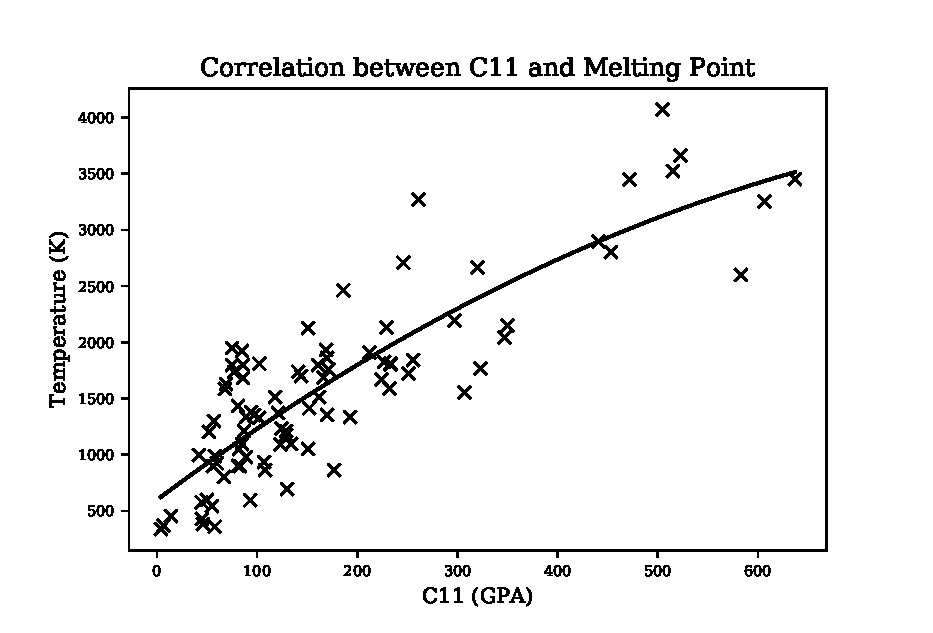
\includegraphics[scale=0.80]{chapters/interatomic_potential_fitting/plots/c11_temperature}%
    \caption{Correlation between $C_{11}$ and temperature}
    \label{fig:c11correlation}
  \end{center}
\end{figure}

The correlation values between the temperature and $C_{11}$ are 0.848 and 0.780 for the Pearsons and Spearmans correlation respectively.  An accurate temperature will not be possible to predict, but it will act as a further sanity check within the computer codes developed in the results section of this work.






